\documentclass{beamer}
\usetheme{Boadilla}
\usepackage{graphicx}
\usepackage[font=small,skip=1pt]{caption}
\captionsetup[figure]{font=small,skip=1pt}

\title{Call Thesis - 29/05/2019}
\author{Matteo Avigni}
\begin{document}
\begin{frame}[plain]
    \maketitle
\end{frame}


\begin{frame}{Agenda}
	\begin{itemize}		
		\item Dataset: meglio partire dal 2016 con tutti i dati o dal 2010 per BTC e dal 2016 per gli altri cripto?
		\item Distribuzione rendimenti: somiglianza BTC con altri asset
	\end{itemize}
\end{frame}
\begin{frame}{BTC prices}
	\begin{figure}[linewidth=250mm]	
		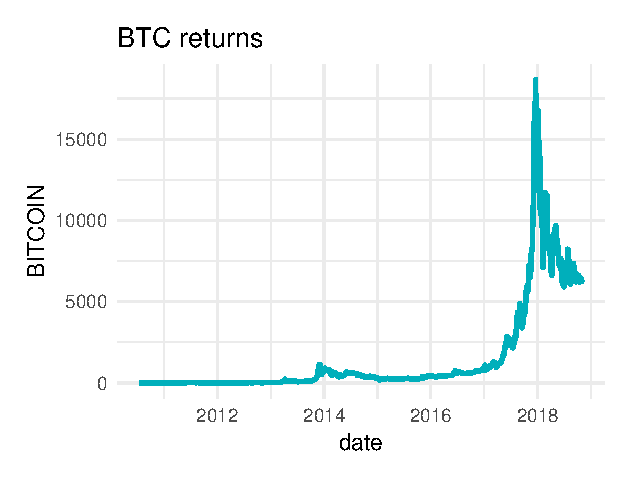
\includegraphics[width=110mm]{BTCprices.eps}
	\end{figure}
\end{frame}
\begin{frame}{BTC returns}
	\begin{figure}[linewidth=250mm]	
		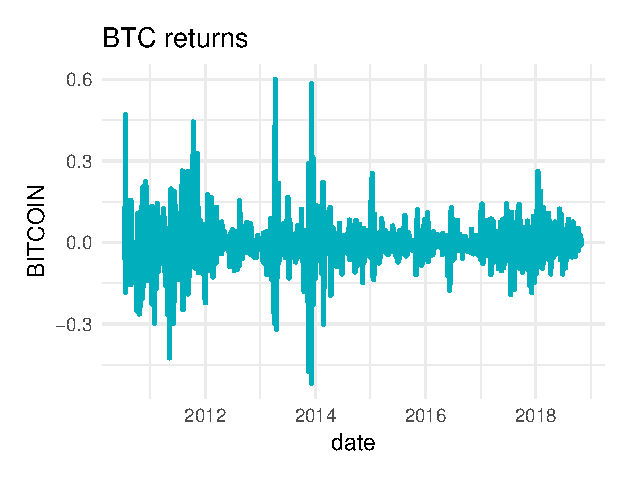
\includegraphics[width=110mm]{BTCreturns.eps}
	\end{figure}
\end{frame}

\begin{frame}{BTC returns qqplot}
	\begin{figure}[linewidth=250mm]	
		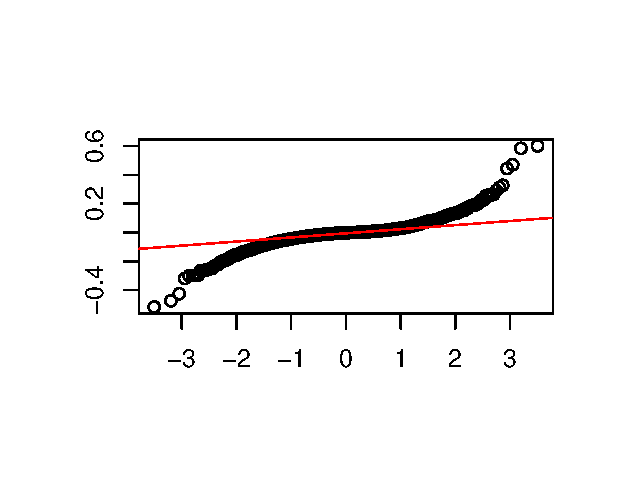
\includegraphics[width=110mm]{BITCOINqqplot.eps}
	\end{figure}
\end{frame}
\begin{frame}{SPX returns qqplot}
	\begin{figure}[b]	
		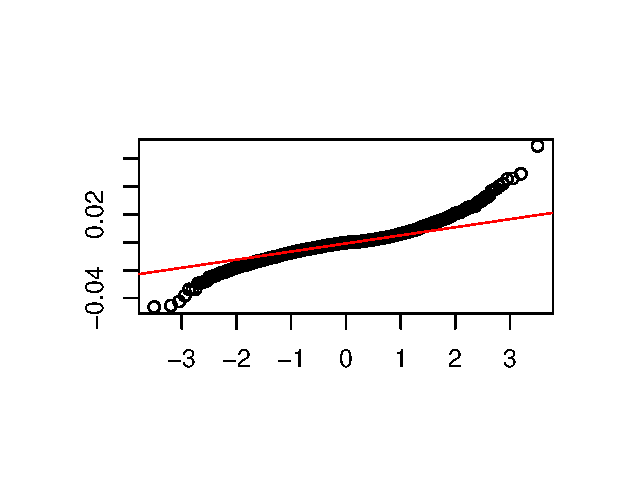
\includegraphics[width=110mm]{S&P500qqplot.eps}
	\end{figure}
\end{frame}
\begin{frame}{QQplots}
	\begin{figure}[h] \label{}
		\begin{minipage}[b]{0.40\linewidth}
			\centering
			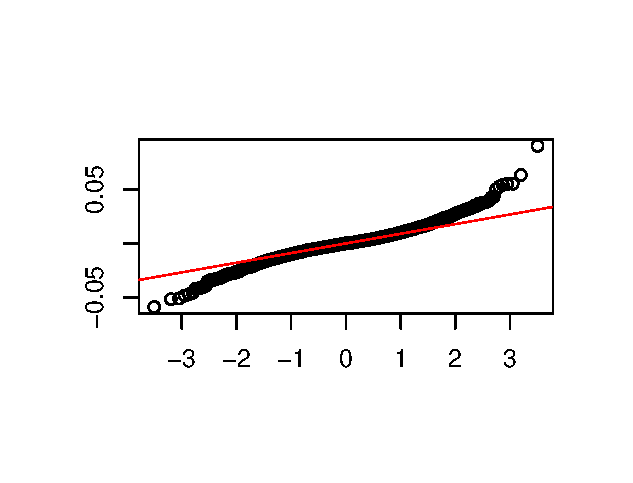
\includegraphics[width=1\linewidth]{EUROSTOXX50qqplot.eps}
			\caption{EUROSTOXX50qqplot}
		\end{minipage} \begin{minipage}[b]{0.40\linewidth}
			\centering
			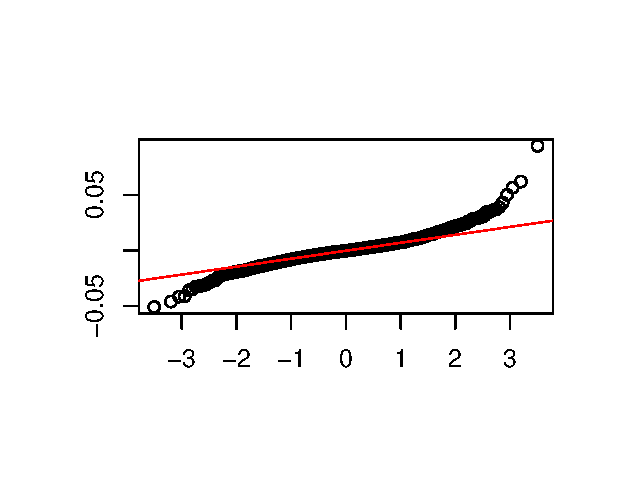
\includegraphics[width=1\linewidth]{GOLDqqplot.eps}
			\caption{GOLDqqplot}
		\end{minipage} \begin{minipage}[b]{0.40\linewidth}
			\centering
			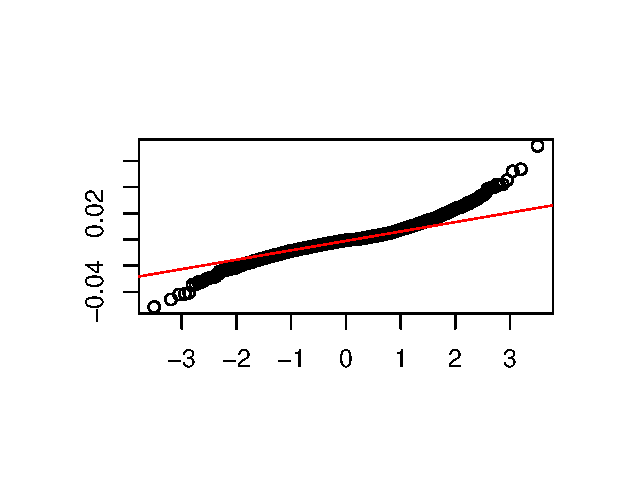
\includegraphics[width=1\linewidth]{NASDAQqqplot.eps}
			\caption{NASDAQqqplot}
		\end{minipage}\hfill
		\begin{minipage}[b]{0.40\linewidth}
			\centering
			\includegraphics[width=1\linewidth]{"VIX Indexqqplot".eps}
			\caption{VIX}
		\end{minipage}
	\end{figure}
	
\end{frame}


\begin{frame}{BTC returns lagplot 1 e 2}
	\begin{figure}[linewidth=250mm]	
		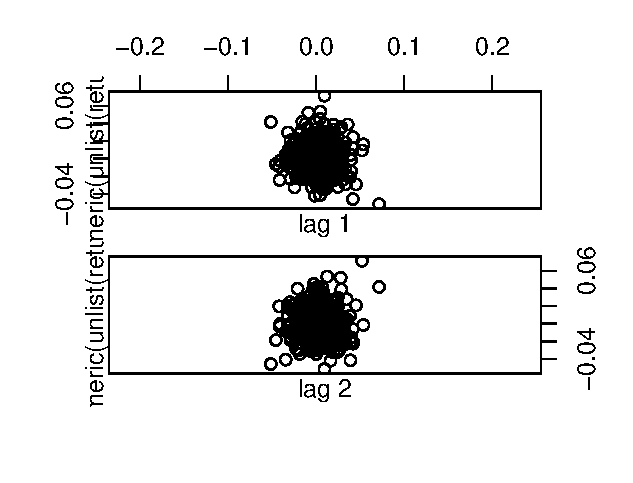
\includegraphics[width=110mm]{BTClagplot2.eps}
	\end{figure}
\end{frame}
\begin{frame}{SPX returns lagplot}
	\begin{figure}[b]	
		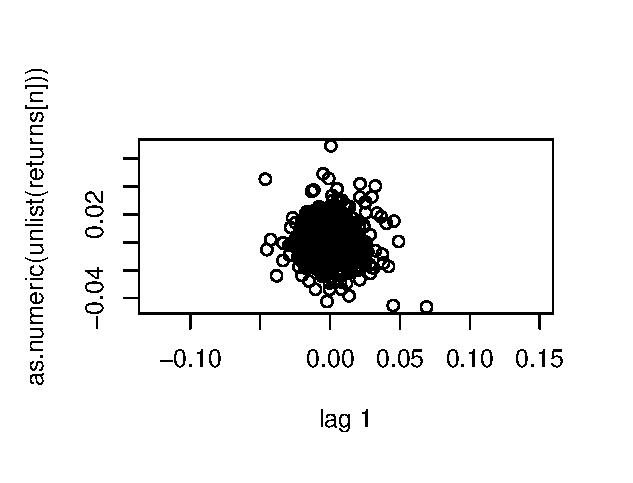
\includegraphics[width=110mm]{S&P500lagplot.eps}
	\end{figure}
\end{frame}
\begin{frame}{lagplots}
	\begin{figure}[h] \label{}
		\begin{minipage}[b]{0.40\linewidth}
			\centering
			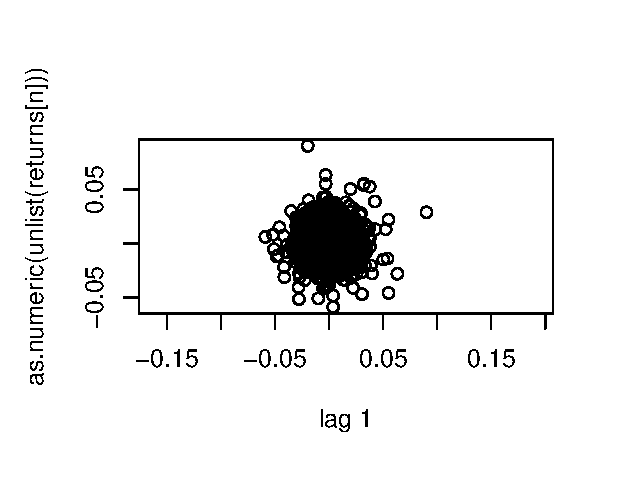
\includegraphics[width=1\linewidth]{EUROSTOXX50lagplot.eps}
			\caption{EUROSTOXX50qqplot}
		\end{minipage} \begin{minipage}[b]{0.40\linewidth}
			\centering
			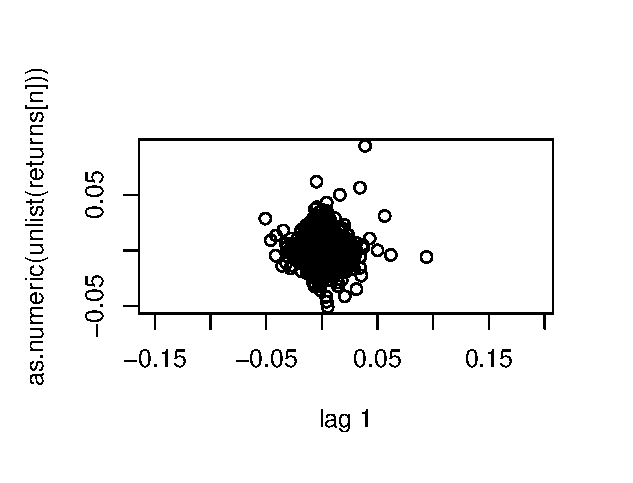
\includegraphics[width=1\linewidth]{GOLDlagplot.eps}
			\caption{GOLDqqplot}
		\end{minipage} \begin{minipage}[b]{0.40\linewidth}
			\centering
			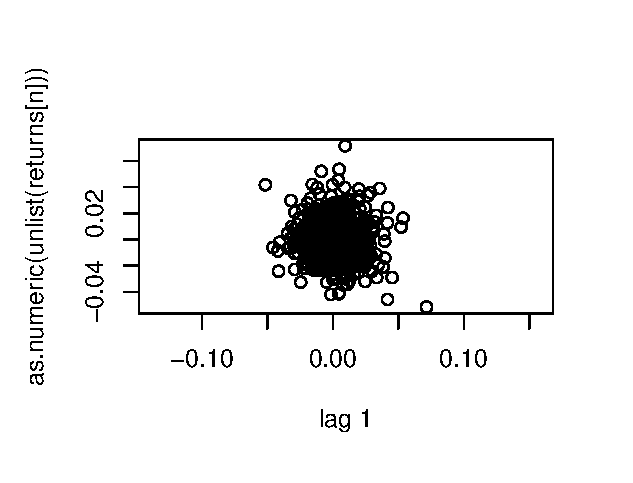
\includegraphics[width=1\linewidth]{NASDAQlagplot.eps}
			\caption{NASDAQqqplot}
		\end{minipage}\hfill
		\begin{minipage}[b]{0.40\linewidth}
			\centering
			\includegraphics[width=1\linewidth]{"VIX Indexlagplot".eps}
			\caption{VIX}
		\end{minipage}
	\end{figure}
	
\end{frame}


\begin{frame}{BTC ACF}
	\begin{figure}[linewidth=250mm]	
		\includegraphics[width=110mm]{BTCacf.eps}
	\end{figure}
\end{frame}
\begin{frame}{SPX acf}
	\begin{figure}[b]	
		\includegraphics[width=110mm]{SPacf.eps}
	\end{figure}
\end{frame}


\begin{frame}{BTCabs ACF}
	\begin{figure}[linewidth=250mm]	
		\includegraphics[width=110mm]{BTCabsacf.eps}
	\end{figure}
\end{frame}
\begin{frame}{SPXabs acf}
	\begin{figure}[b]	
		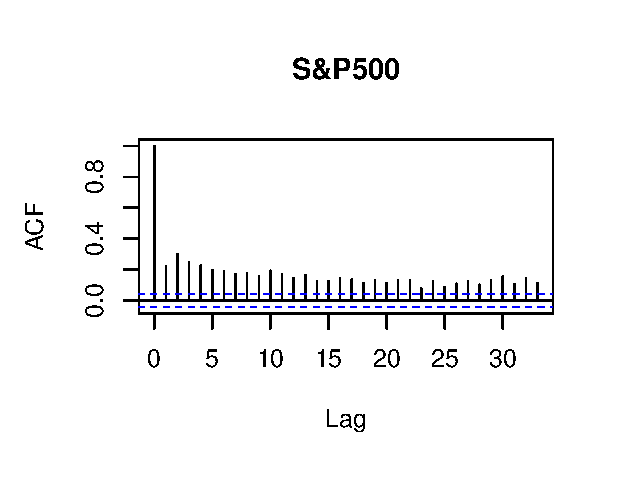
\includegraphics[width=110mm]{SPabsacf.eps}
	\end{figure}
\end{frame}



\begin{frame}{Conclusioni}
	\begin{itemize}
		\item Rendimenti bitcoin modellizzabili come gli altri rendimenti, solo con volatilità maggiore
		\item GARCH?
	\end{itemize}
\end{frame}

\end{document}
